The aim of this procedure is the estimation of the median spectral acceleration value $\hat{S}_{a,ds}$, that brings the structure to the attainment of a set of damage states ds, and the corresponding dispersion beta $\beta_{S_a}$, the parameters needed for the mathematical representation of fragility in equation \ref{eq:fragility-definition}. The aim is achieved making use of the tool spo2ida (Vamvatsikos and Cornell, 2006), where static pushover curves are converted into 16\%, 50\% and 84\% IDA curves, using empirical relationships from a large database of incremental dynamic analysis results, as shown in Figure~\ref{fig:spo2ida}.

\begin{figure}[H]
\centering
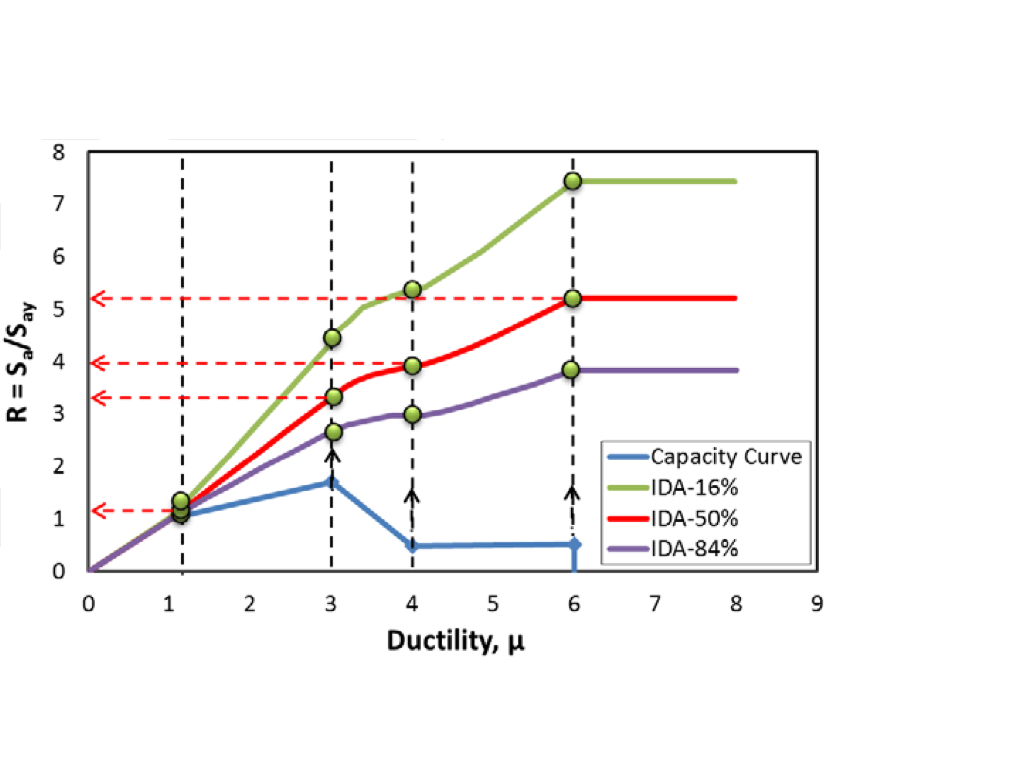
\includegraphics[width=12cm,height=8cm]{./figures/spo2ida.jpg}
\caption{spo2ida tool: IDA curves derived from Pushover curve.}
\label{fig:spo2ida}
\end{figure}

The spo2ida-based procedure presented herein is applicable to any kind of multi-linear capacity curve, and it is suitable for single building fragility curve estimation, as described in section \ref{subsubsec:single-building-spo2ida}. However the fragility curves derived for single buildings can be combined in a unique fragility curve, which considers the inter-building uncertainty, as described in section \ref{subsubsec:multiple-building-spo2ida}.

\subsubsection{Single-building Fragility and Vulnerability function}
\label{subsubsec:single-building-spo2ida}
Given the idealised capacity curve the spo2ida tool uses an implicit R-$\mu$-T relation to correlate nonlinear displacement, expressed in terms of ductility $\mu$ to the corresponding medians capacity in terms of the parameters R. R is the lateral strength ratio, defined as the ratio between the spectral spectral acceleration S$_a$ and the yielding capacity of the system S$_{ay}$. 

Each branch of the capacity curve, hardening, softening and residual plateau, is converted to a corresponding branch of the three ida curves, using the R-$\mu$-T relation, which is a function of the hardening stiffness, the softening stiffness and the residual force. These parameters are derived from the idealised pushover capacity expressed in $\mu$-R terms, as well as the ductility levels at the onset of each branch. If some of the branches of the pushover curve are missing because of the seismic behaviour of the system, spo2ida can equally work with bilinear, trilinear and quadrilinear idealisations.

The result of the spo2ida routine is thus a list of ductility levels and corresponding R values at 50\%, 16\% and 84\% percentiles. The distribution of R values at each ductility level, due to the record-to-record variability, is assumed to be lognormal and it can be easily converted to the dispersion of the lognormal distribution with the following equation:

\begin{equation}
\beta_{R(\mu)} = \frac{\ln R(\mu)_{84\%} - \ln R(\mu)_{16\%}}{2}
\label{eq:betaR}
\end{equation} 

$\beta_{R(\mu)}$ represents also the record-to-record variability of S$_a$ at different ductility levels $\beta_{S_a, d}$. Median R and its dispersion at ductility levels corresponding to the damage thresholds can thus be determined, and $\hat{S}_{a,ds}$ can be easily extracted simply multiplying $R_{50\%}(\mu_{ds})$ by the yielding capacity of the system $S_{ay}$, as shown in the following equation:

\begin{equation}
\hat{S}_{a,ds} = R_{50\%}(\mu_{ds}) S_{ay}
\label{eq:SaR}
\end{equation}
\begin{equation}
S_{ay} = \frac{4 \pi^2 \delta_{roof,y}}{g \Gamma_1 T_1^1}
\end{equation}

Since $\hat{R}$ and $\hat{S}_{a}$ are proportional they share the same dispersion.

If dispersion due to uncertainty in the limit state definition $\beta_{\theta c}$ is different from zero it can not be combined directly with the record-to-record dispersion, but a Monte Carlo sampling of the limit state needs to be performed instead. Different values of ductility limit state are sampled from the  lognormal distribution with median the median value of the ductility limit state, and dispersion the input $\beta_{\theta c}$. For each of these ductilities the corresponding R$_{16\%}$-R$_{50\%}$-R$_{84\%}$ are found and converted into $\hat{S}_{a,ds}$ and $\beta_{\theta d}$ according to equation \ref{eq:SaR} and \ref{eq:betaR}. N random S$_a$ corresponding to the N sampled ductility limit states are computed, and their median and the dispersion are estimated. These parameters constitute the median $\hat{S}_{a,ds}$ and the total dispersion $\beta_{S_a}$ for the considered damage state. The procedure is repeated for each damage state.

To derive a discrete vulnerability function at certain intensity measure levels, the input damage-to-loss factors are applied to the probability of occurance of each damage state, extracted from the probability of exceedance of each damage state described by the set of fragility curves. 

If dispersion due to uncertainty in the limit state is different from zero a vulnerability function is derived for the N sets of sampled ductility limit states. It results in N loss ratios for each defined intensity measure levels. Finally a lognormal distribution of the loss ratios is assumed at each iml and the vulnerability curve is defined at each iml by the mean and the standard deviation of all the computed loss ratios.

\subsubsection{Multiple-Building Fragility and Vulnerability function}
\label{subsubsec:multiple-building-spo2ida}
If multiple buildings have been input to derive a set of fragility curves for a class of buildings all $\hat{S}_{a,blg}$ and $\beta_{S_a,blg}$ are combined in a single lognormal curve for each damage state. A minimum of 5 buildings should be considered to obtain reliable results for the class. The procedure to get $\mu_{S_a,tot}$ and $cov_{S_a,tot}$ for the class of building is the same described in section \ref{subsubsec:multiple-buildings}, but the $\hat{S}_{a,blg}$ and $\beta_{S_a,blg}$ are those derived from each sampled set of ductility limit state.

A single vulnerability curve can also be obtained, from the single building vulnerability curves. If no dispersion in the limit state is defined, the method is the same described in section \ref{subsubsec:multiple-buildings}. Otherwise a vulnerability curve is derived for each building as explained in section \ref{subsub:single-building-spo2ida}, considering the sampled set of ductility limit states, that is to say that the mean loss ratio and its standard deviation at each iml, $\mu_{LR,iml,blg}$ and $\sigma_{LR,iml,blg}$ respectively, are found for each building.
Finally the mean loss ratio and its standard deviation, $\mu_{LR,iml}$ and $\sigma_{LR,iml}$, are found for the entire class of buildings as the weighted mean of the single $\mu_{LR,iml,blg}$ and the weighted SRSS of the inter-building and intra-building standard deviation, the standard deviation of the single means $\mu_{LR,iml,blg}$ and the single dispersions $\sigma_{LR,iml,blg}$ respectively, as described in eq \ref{eq:combination-lognormals-sigma}, substituting loss ratio to spectral acceleration.

\subsubsection{Inputs}
\label{subsubsec:InputSpo2ida}
The inputs must be formatted as comma-separated value files (.csv), and saved in the folder \textit{input}, contained in the NSP directory. If any other environment different from Windows is used make sure that the "comma separated values Windows" is selected as saving option when creating the input files. 

If multiple buildings want to be analysed to consider the inter-building uncertainty the parameters relative to each building should be added as additional lines in the tables, as shown in the examples below, otherwise a single line must be input.

If the user has already at disposal an idealised multilinear pushover curve for each building, that is to say that the variable \textit{in\_type} has been set to 0, the following data need to be provided in the corresponding csv files:

\begin{enumerate}
\item First period of vibration $T_1$, corresponding modal participation factor $\Gamma_1$, normalised with respect to the roof displacement, and weight for the combination of different buildings, input in \textit{building\_parameters.csv}, as in section \ref{subsubsec:InputCr}, input n. 1.
	
\item Top displacement at each damage state threshold and corresponding dispersion $\beta_{\theta c}$ input in \textit{displacement\_profile.csv}, as in section \ref{subsec:InputCr}, input n. 2. 
	
\item Idealised pushover curve, input in \textit{idealised\_curve.csv} as shown below. The parameters needed to describe the idealised pushover curve are: yielding displacement d$_y$, displacement at the onset of degradation d$_s$, displacement at the onset of residual force d$_{min}$, ultimate displacement d$_u$, maximum force F$_{max}$, residual force F$_{min}$. These parameters are represented in Figure~\ref{fig:quadrilinear}.

\begin{figure}[H]
\centering
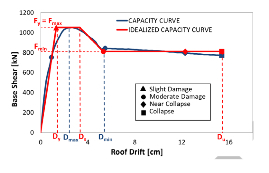
\includegraphics[width=12cm,height=8cm]{./figures/quadrilinear.jpg}
\caption{Idealisation of capacity curve using multilinear elasto-plastic form.}
\label{fig:quadrilinear}
\end{figure}

\begin{table}[H]
\centering
\begin{tabular}{|c|c|c|c|c|c|c|} \hline
\textbf{n.building} & \textbf{d$_y$} & \textbf{d$_s$} & \textbf{d$_{min}$} & \textbf{d$_u$} & \textbf{F$_{max}$} & \textbf{F$_{min}$} \\ \hline
1 & 0.09	& 0.3	& a & b & 523 & 430\\ \hline
2 & 0.12	& 0.35	 & a & b & 400 & 305\\ \hline	
\end{tabular}
\end{table}

\item Consequence model (loss ratio per each damage state) consistent with the defined set of damage states, input in \textit{consequence.csv}, as in section \ref{subsubsec:InputCr}, input n. 5.
	
\end{enumerate}

If these data are not available, \textit{in\_type} = 0 can be selected and the "raw" results from a pushover analysis can be input instead. The same data as in section \ref{subsubsec:InputCr} for \textit{in\_type} = 0 can be input.

\subsubsection{Calculation Steps}
The overall workflow of spo2ida-based procedure is summarised in this section. The option \textit{an\_type} must be set equal to 1 and the option \textit{in\_type} according to the input at disposal. The corresponding inputs should follow the requirements described in section \ref{subsec:InputSpo2ida}. At this point the code proceeds with the following steps:

\begin{enumerate}
\item 
\begin{enumerate}
\item If \textit{in\_type} = 0, the roof displacement at each limit state and the idealised pushover curve parameters are extracted from \textit{displacement\_profile.csv} and \textit{idealised\_curve.csv} respectively.

\item If \textit{in\_type} = 1 the results from a pushover analysis are extracted from \textit{displacements\_pushover.csv} and \textit{reactions\_pushover.csv} and drift limit states from {limits.csv}. The idealised pushover curve is then derived in the \textit{idealisation} function, where the idealisation process is conducted according to the Gem Analytical Vulnerability Guidelines.	\end{enumerate}

\item The parameters extracted are used to derive ductility levels $\mu_{ds}$, median spectral acceleration $\hat{S}_{a,ds}$ and the total dispersion $\beta_{S_a}$ at each damage threshold through the following steps:
\begin{itemize}
\item The idealised MDoF system is transformed into an equivalent SDoF system, using $\Gamma_1$, and SDoF capacity curve is  expressed in terms of $\mu$-R.

\item The variables for spo2ida tool are extracted from the capacity curve and they are used as input to get the 16\%-50\%-84\% ida curves.

\item The ductility levels $\mu_{ds}$ corresponding to each damage threshold are defined, and the corresponding R$_{16\%}$-R$_{50\%}$-R$_{84\%}$ are found in ida outputs.

\item $\hat{S}_{a,ds}$ and the corresponding dispersion $\beta_{S_{a, d}}$ are computed using eq.~\ref{eq:SaR} and eq.~\ref{eq:betaR}, respectively.

\item If dispersion due to uncertainty in the limit state $\beta_{\theta c}$ is different from zero different ductility limit states are sampled for each median ductility level $\mu_{ds}$ and corresponding values of $\hat{S}_{a,ds}$ and $\beta_{S_{a, d}}$ are computed, as described in section \ref{subsubsec:single-building-spo2ida}, but not yet combined together.

\end{itemize}

\item All $\hat{S}_{a, ds}(T_1)$ are converted to mean $\mu_{ln(S_{a, ds})}(T_1)$ and then to the intensity measure in common with the rest of the buildings, $\mu_{ln(S_{a, ds}(T_{av}))}$, according to eq. \ref{eq:Sa(Tav)}.

\item Step 2. and 3. are repeated for the number of input buildings.

\item
\begin{enumerate}

\item If vulnerability = 0: All $\hat{S}_{a,ds}$ and $\beta_{S_{a, d}}$ from all the buildings and all the sampled ductility limit states are combined in a single lognormal curve, as described in section \ref{subsubsec:single-building-spo2ida}. 
Mean $\mu_{ln(S_{a})}$ and total dispersion $\beta_{S_a}$ are then converted to logarithmic mean $\mu_{S_a}$ and logarithmic covariance $cov_{S_a}$, according to equations \ref{eq:median-to-mean} and \ref{eq:dispersion-to-standard} respectively.
Fragility curves for the class of buildings are displayed if the variable \textit{plotflag}[2] = 1, and logarithmic $\mu_{S_a}$ and $cov_{S_a}$ are exported in the \textit{outputs} folder.
\item If vulnerability =1:  
For the intensity measure levels defined in the variable \textit{iml} a value of loss ratio $\mu_{LR, iml, blg}$ is defined for each building and a standard deviation $\sigma_{LR, iml, blg}$, if dispersion due to uncertainty in the limit state $\beta_{\theta c}$ is different from zero. They are finally combined in a single mean and standard deviationas described in section \ref{subsubsec:multiple-building-spo2ida}. Vulnerability curve for the class of buildings is displayed if the variable \textit{plotflag}[3] = 1, and $\mu_{LR}$ and $cov_{LR}$ at each iml are exported in the \textit{outputs} folder.
\end{enumerate}

\end{enumerate}